In this subsection it is explained which microservices will be custom and which one will be used as pay-per-use. 
\\All microservices will be stored in the Cloud offered by IBM and every microservice is picked from the IBM Cloud Platform.
\\For services that are used with the pay-as-you-go mechanism it is briefly explained how they work and some diagrams are included to better understand the concept.
\begin{itemize}
	\item \textbf{Login - \href{https://cloud.ibm.com/catalog/services/app-id}{IBM App ID}}: This microservice is about User Authentication and Management, and provides a log-in framework. App ID will be used to add authentication to our web and mobile apps securing our Cloud-native applications and services on IBM Cloud. By requiring users to sign in to our app, we will be able to store user data such as app preferences or information from public social profile to recognize user that reports violations and customize each user's experience within the app.
	\\When a user is successfully authenticated, the application receives tokens from App ID. The service uses three main types of tokens to complete the authentication process: Access Token, Identity Token and Refresh Token.
	\begin{figure}[h!]
		\makebox[\textwidth]{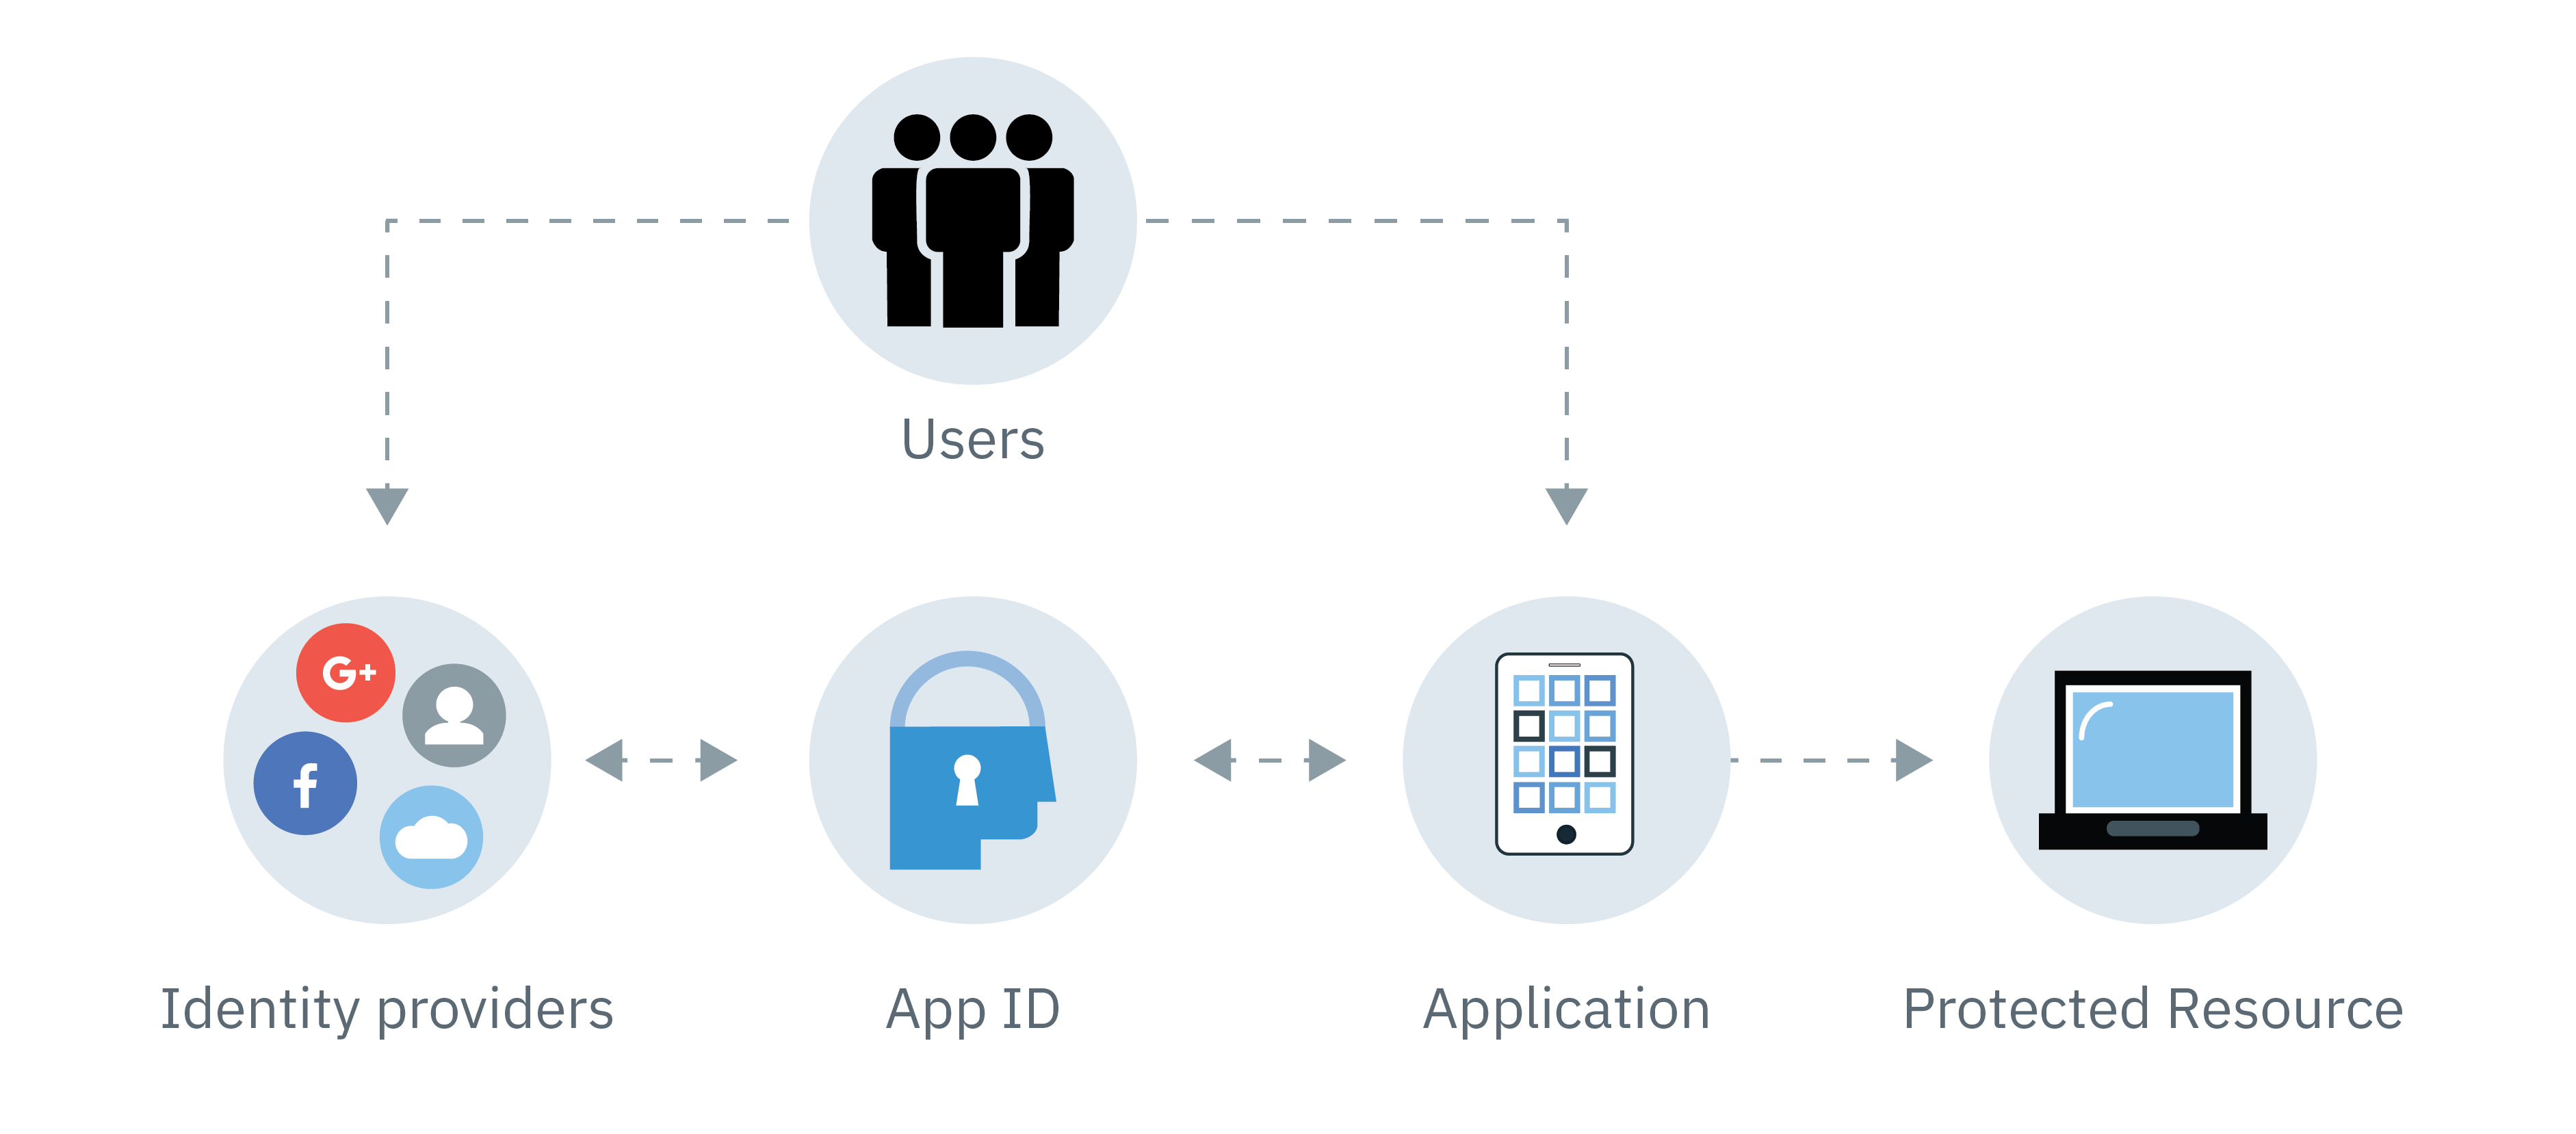
\includegraphics[width=1.15\textwidth]{/images/microservices/appidarchitecture.png}}
		\caption{IBM App ID working diagram.}
	\end{figure}
	\FloatBarrier

	\item \textbf{Computer Vision - \href{https://cloud.ibm.com/catalog/services/visual-recognition}{IBM Watson Visual Recognition}}: This service uses deep learning algorithms to analyze images for scenes, objects, and other content. In our scenario it will be used for certifying automatic tickets and to extract various information from violation's pictures.
	\\Its usage is simple as making an HTTP request to its POST API sending the image then wait for it to finish his work. The response that it returns includes keywords that provide information about the content along with an estimate probability of them being identified.
	\\In addition, IBM Watson Visual Recognition supports high availability with no single point of failure. Recovering from potential disasters that affect an entire IBM location requires planning and preparation but can always be done saving all of our custom training model.
	\begin{figure}[h!]
		\makebox[\textwidth]{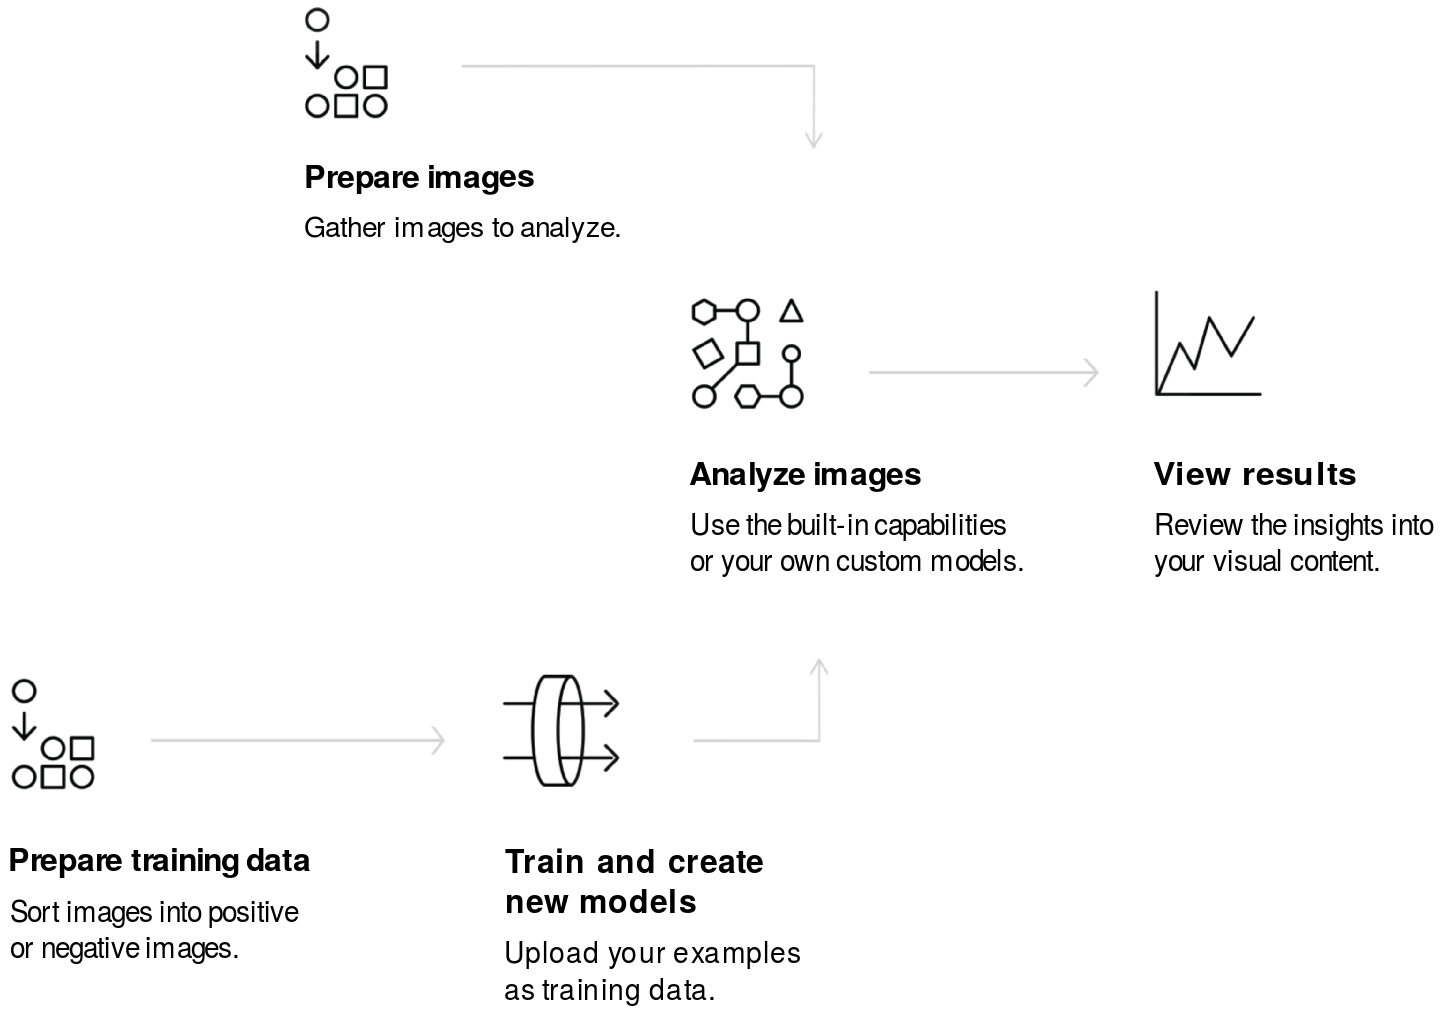
\includegraphics[width=1.15\textwidth]{/images/microservices/visualrecognition.png}}
		\caption{IBM Watson Visual Recognition working diagram.}
	\end{figure}
	\FloatBarrier
	
	\item \textbf{Data Mining - \href{https://cloud.ibm.com/catalog/services/discovery}{IBM Watson Discovery}}: IBM Watson Discovery makes it possible to rapidly build cognitive, cloud-based exploration applications that unlock insights hidden in unstructured data. 
	\\This microservice is particularly useful when, at a given time everyday, SafeStreets crosses data coming from the municipality with its own data to extract potential suggestions.
	\\With Discovery, it only takes a few steps to prepare our unstructured data coming from different sources and to create a query that will pinpoint the information SafeStreets needs. Discovery automatically uses data analysis combined with cognitive intuition to take the unstructured data and enriches it to discover hidden information.
	\begin{figure}[h!]
		\makebox[\textwidth]{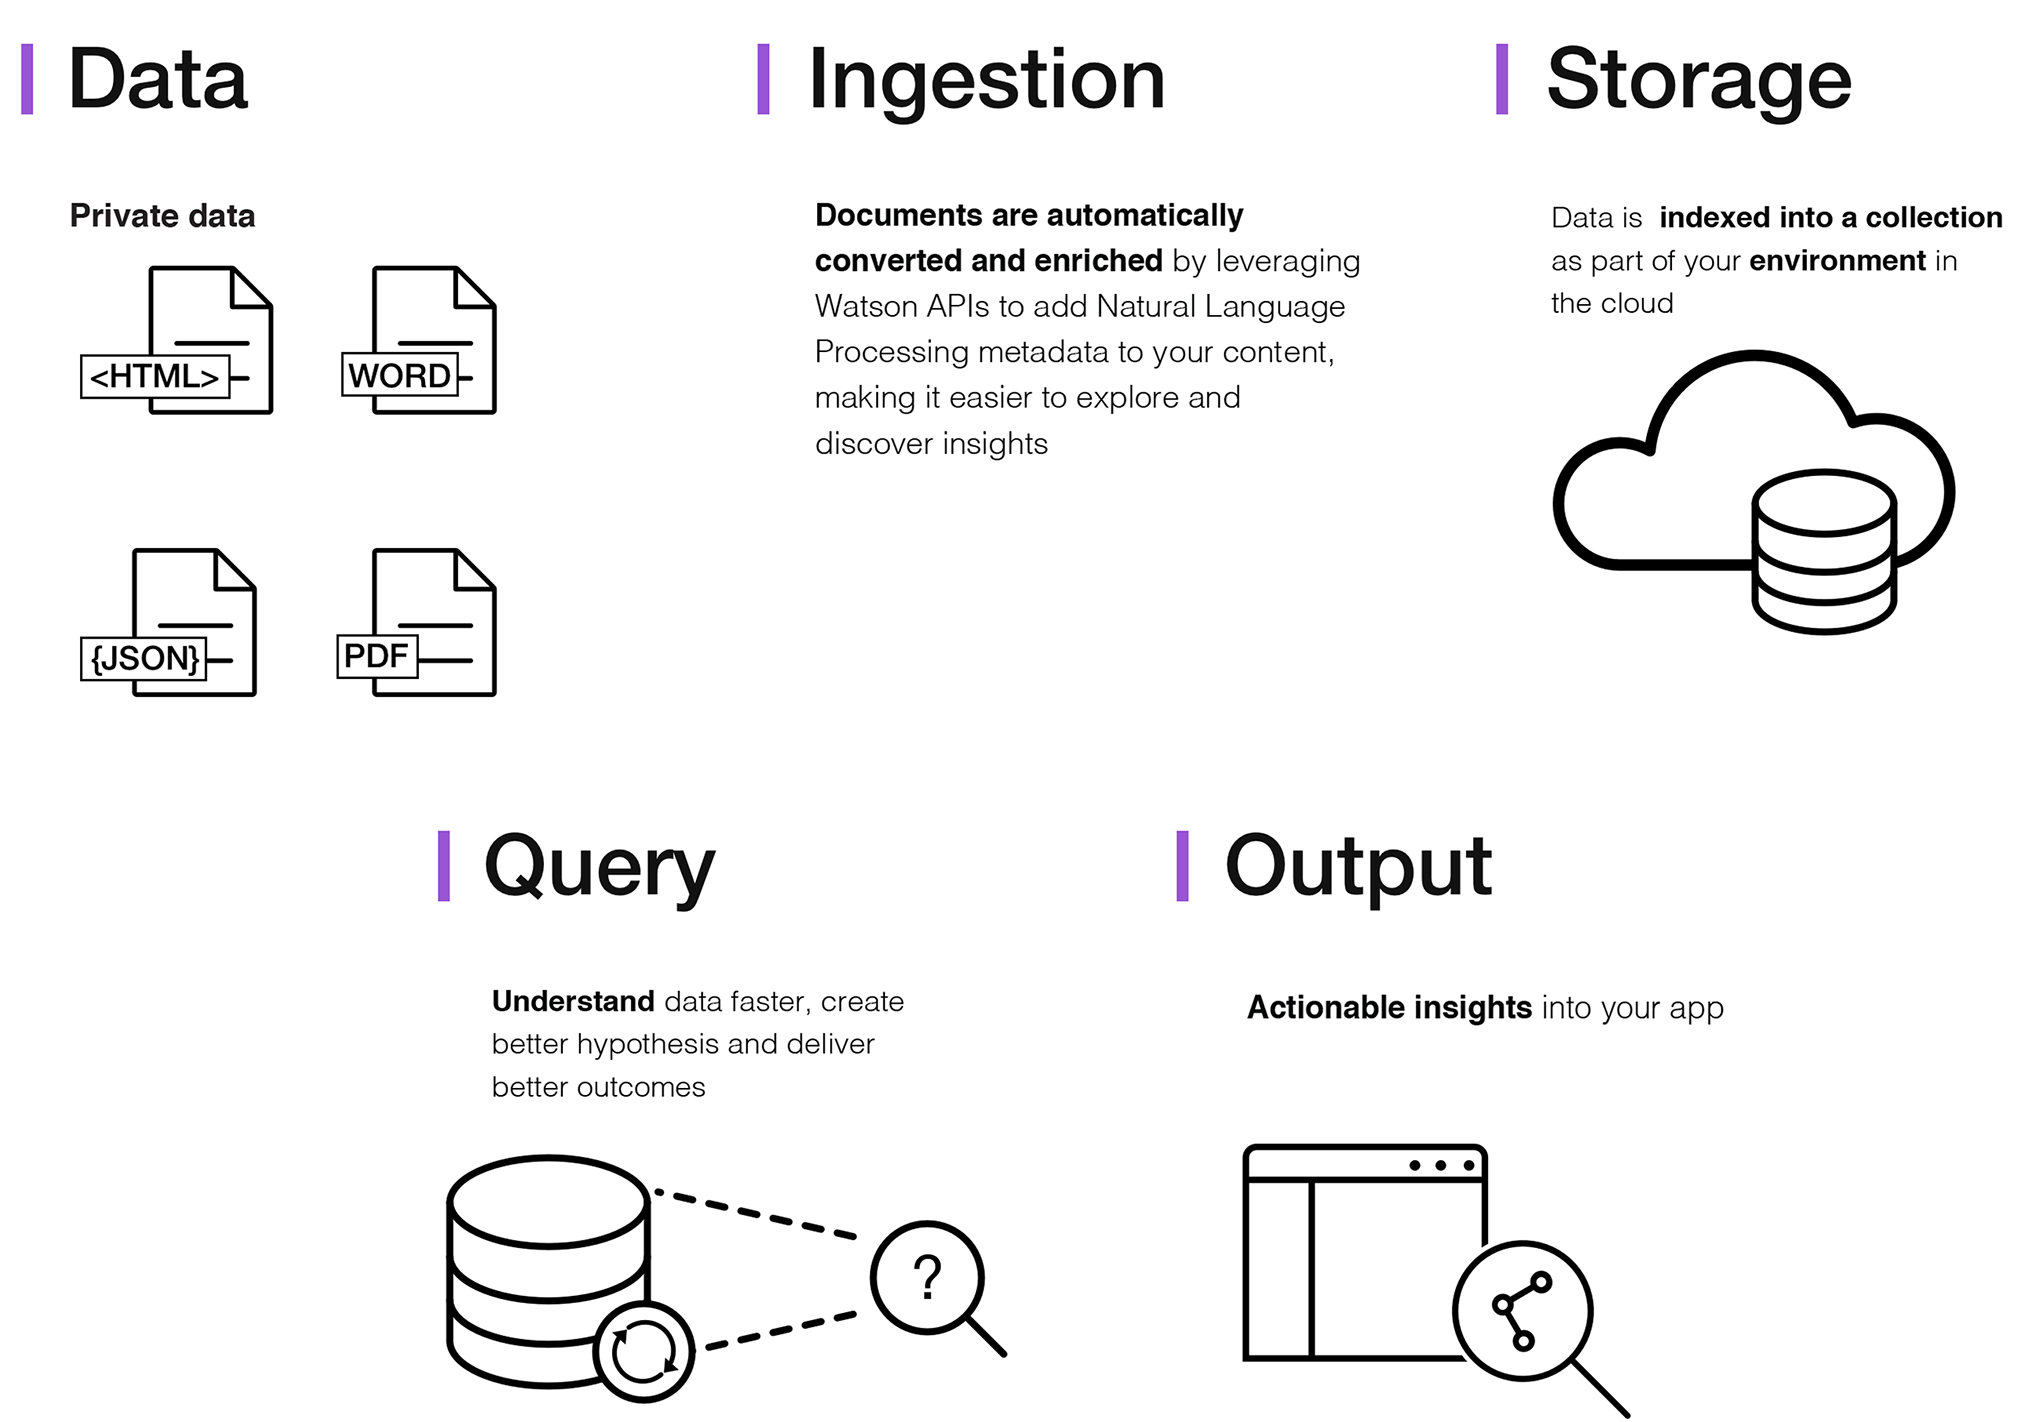
\includegraphics[width=1.25\textwidth]{/images/microservices/discoveryflow.png}}
		\caption{Complete architecture of our Discovery solution.}
	\end{figure}
	\FloatBarrier
	
\end{itemize}